%
% File acl2012.tex
%
% Contact: Maggie Li (cswjli@comp.polyu.edu.hk), Michael White (mwhite@ling.osu.edu)
%%
%% Based on the style files for ACL2008 by Joakim Nivre and Noah Smith
%% and that of ACL2010 by Jing-Shin Chang and Philipp Koehn


\documentclass[11pt,letterpaper]{article}
\usepackage[letterpaper]{geometry}
\usepackage{acl2012}
\usepackage{times}
\usepackage{latexsym}
\usepackage{amsmath}
\usepackage{multirow}
\usepackage{graphicx}
\usepackage{url}
\makeatletter
\newcommand{\@BIBLABEL}{\@emptybiblabel}
\newcommand{\@emptybiblabel}[1]{}
\makeatother
\usepackage[hidelinks]{hyperref}
\DeclareMathOperator*{\argmax}{arg\,max}
\setlength\titlebox{6.5cm}    % Expanding the titlebox

\title{Neural and Symbolic Arabic Paraphrasing with Automatic Evaluation}

\author{First Author \\
  Affiliation / Address line 1 \\
  Affiliation / Address line 2 \\
  Affiliation / Address line 3 \\
  {\tt email@domain} \\\And
  Second Author \\
  Affiliation / Address line 1 \\
  Affiliation / Address line 2 \\
  Affiliation / Address line 3 \\
  {\tt email@domain} \\\And
  Weijian Lin \\
 Carnegie Mellon University\\
 School of Computer Science \\ 
 5000 Forbes Avenue, Pittsburgh, PA 15213 \\
  {\tt wlin1@cs.cmu.edu} \\}

\date{}

\begin{document}
\maketitle
\begin{abstract}

	We present a tool for Arabic paraphrasing that yields good paraphrasing accuracy.  We present and compare several methods for paraphrasing and obtaining monolingual parallel data. We also present first results on Arabic paraphrasing using neural methods. Additionally, we propose a new evaluation metric for paraphrasing that is shown to correlate highly with human judgement.
\end{abstract}


\section{Introduction}

\section{Related Work}

\section{Obtaining Parallel Monolingual Data}

\section{Extracting Paraphrases}
Our first approach to Arabic paraphrasing is the pivot method proposed by Bannard and Callison-Burch\cite{bannard2005bilingual}. A key benefit is that it is language-agnostic and is based on the idea that any two source strings $e_1$ and $e_2$ that both translate to a reference string $f_1$ have similar meaning. Bannard and Callison-Burch used English as the reference string $f$, but in our study we will instead pivot into English to obtain paraphrase pairs. We obtain the final paraphrase probability by marginalizing over the English translation probabilities with $e$ and arabic phrases $a_1$ and $a_2$. A mathematical formulation of the approach can be found in Equation 1.

\begin{equation}
p(a_2 | a_1) = \sum_{e} p(a_2 | e) p(e | a_1)
\end{equation}

In order to extract paraphrases, we first obtained a parallel bilingual corpus through English and Arabic versions of the EUROPARL dataset \cite{Koehn_europarl}. We 
\begin{figure*}
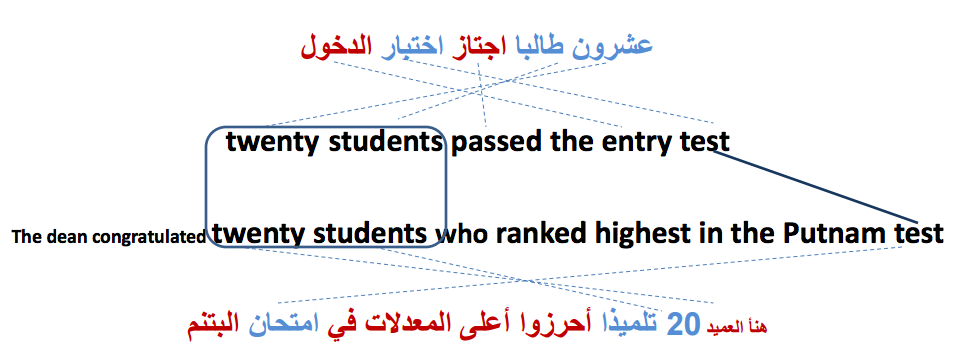
\includegraphics[scale=0.5]{arabic_pivot}
\caption{An example paraphrased sentence produced using the pivot method. }
\end{figure*}
\section{Generating Paraphased Sentences}
	To address the shortage problem for Arabic language data, here we propose a novel method for generating Arabic parallel language sentences using other two languages pairs as resource. The idea is to use paired sentences data from two other languages, translate them into Arabic correspondingly, then use them as the  training data for sequence to sequence machine translation model to train a translator  to generate Arabic to Arabic paraphrases.
  
	The first advantage of this approach is its scalability. After preparing enough training data for the paraphraser model, the generation step for Arabic paraphrases is easily scalable. The second advantage is that paraphraser model may contain valuable insight for  building Arabic paraphrases database at  words and phrases level, since state of the art neural machine translation techniques are capable of capturing word and phrase level similarity by projecting word embeddings into vector space.
	
	We use europarl-v7.fr-en data which contains two millions sentence pairs, and then use Google translate API to generate French-Arabic and English-Arabic sentence pairs correspondingly. Then we use them as training data to train a single layer sequence to sequence attentional encoder-decoder model, with embedding size and hidden size set to be 512 while attention size set to be 128. The whole process is demonstrated in the following  \ref{figure1}

\subsection{Phrase Substitution Method}
\subsection{Neural Seq-to-Seq Method}

\section{An Automatic Evaluation Metric}
\subsection{Semantic Similarity}	
\subsection{Surface Variation}

\section{Analysis}

\section{Evaluation}

\section{Future Work}
 We plan to explore other options for obtaining monolingual parallel data. One possible approach is to retrieve headlines of news articles from different agencies covering the same event. We expect headlines describing the same event to have some degree of semantic similarity yet different surface realizations.\\
 The sequence-to-sequence models required a relatively long time to run which limited the testing of other architectures and model options. We plan to conduct more experiments on different architectures and compare results.  





\section*{Acknowledgments}

\bibliography{projectreport}
\bibliographystyle{acl2012}

\end{document}


